\section{Vrify - A design toolbox for VR}
Based on the results from the interviews and the theoretical framework, a toolbox for creative processes and design of VR applications were created. The toolbox were designed based on simple user stories and scenarios. Specifications of the controllers and buttons that are referenced in this section can be found in section \ref{result:hardware}.

\subsection{Lo-Fi Prototypes}
 Several different sketches and concepts were created to obtain a diversity of interfaces to test. A lo-fidelity prototype was developed with these sketches as a foundation, these were later evaluated with simple testing rounds. The concepts and elements in this section where selected for the Hi-fi prototyping phase after these tests.

\subsubsection{Main interface - Belt UI}
The main interface is designed for the users ergonomic position when seated, displayed from the hip of the user.(Figure \ref{fig:lofi:belt-ui}) The main purpose of this interface is to create a new object and place them into the world (Figure \ref{fig:lofi:belt-ui:add}), as well as to change properties of selected object/objects (Figure \ref{fig:lofi:belt-ui:props}). The centered feature in this UI is the scene-hierarchy, from where objects can be selected and created. The purpose of this approach is to introduce the hierarchy to the user as the starting point of the process. The users FOV will look like an extension of a work-bench (Figure \ref{fig:lofi:fov:belt-ui}), and can be accessed by pressing the application-button on the controller.

\subsubsection{UI Selectors}
\label{result:lofi:selector}
A selector UI (building from work in section \ref{theory:toolsandtech:selector}) is used to manipulate and interact with objects. As seen in Figure \ref{fig:lofi:fov:selector}, the selector appears next to an object that has been selected and offers actions that are targeted to the selected object. The UI is designed as a pie-menu (Figure \ref{fig:lofi:selector:select}) that grants the oppertunity one level of sub-menus (Figure \ref{fig:lofi:selector:submenu}). The selector UI is accessed through the touchpad on the controller (for hardware specs, see section \ref{theory:hardware:controllers}).

\subsubsection{Object selection and manipulation}
Interactions and sequences for selecting and manipulating objects (Figure \ref{fig:lofi:object}) are explained here as scenarios.
\begin{itemize}
  \item \textbf{Selecting an object:} The user points the controller towards object, so that the raycast hits it. Then the user clicks the selection-button to select the targeted object.
  \item \textbf{Moving an object} When the user selects the object, a bounding-box becomes visible around the object along with three axis' and a grid (Figure \ref{fig:lofi:belt-ui:props}). By targeting the bounding-box and holding the selection-button the user can now use the raycast to position the object along the grid. If the user wants to move the object in the third dimension (that is not covered by the grid), grab the grid in a similar fashion and use the raycast to move. It's state is movable by default. Unless changed in the selector UI (section \ref{result:lofi:selector}), it can be moved straight away. The axis' of the grid can be changed using the selector UI.
\end{itemize}


\subsubsection{Tilt-Brush Tests}
Concepts that made it through initial testing were drawn in Tilt Brush (see Figure \ref{fig:lofi:tilt}) in order to visulize how perspectives and field of view works with the concept in VR.

**Missing section: Explaination**

%% ********* BELT UI IMAGES **********

\begin{figure}
\begin{subfigure}{.5\textwidth}
  \centering
  \includegraphics[width=.8\linewidth]{lo-fi/belt-add.jpg}
  \caption{Properties of a selected object in the belt UI}
  \label{fig:lofi:belt-ui:props}
\end{subfigure}%
\begin{subfigure}{.5\textwidth}
  \centering
  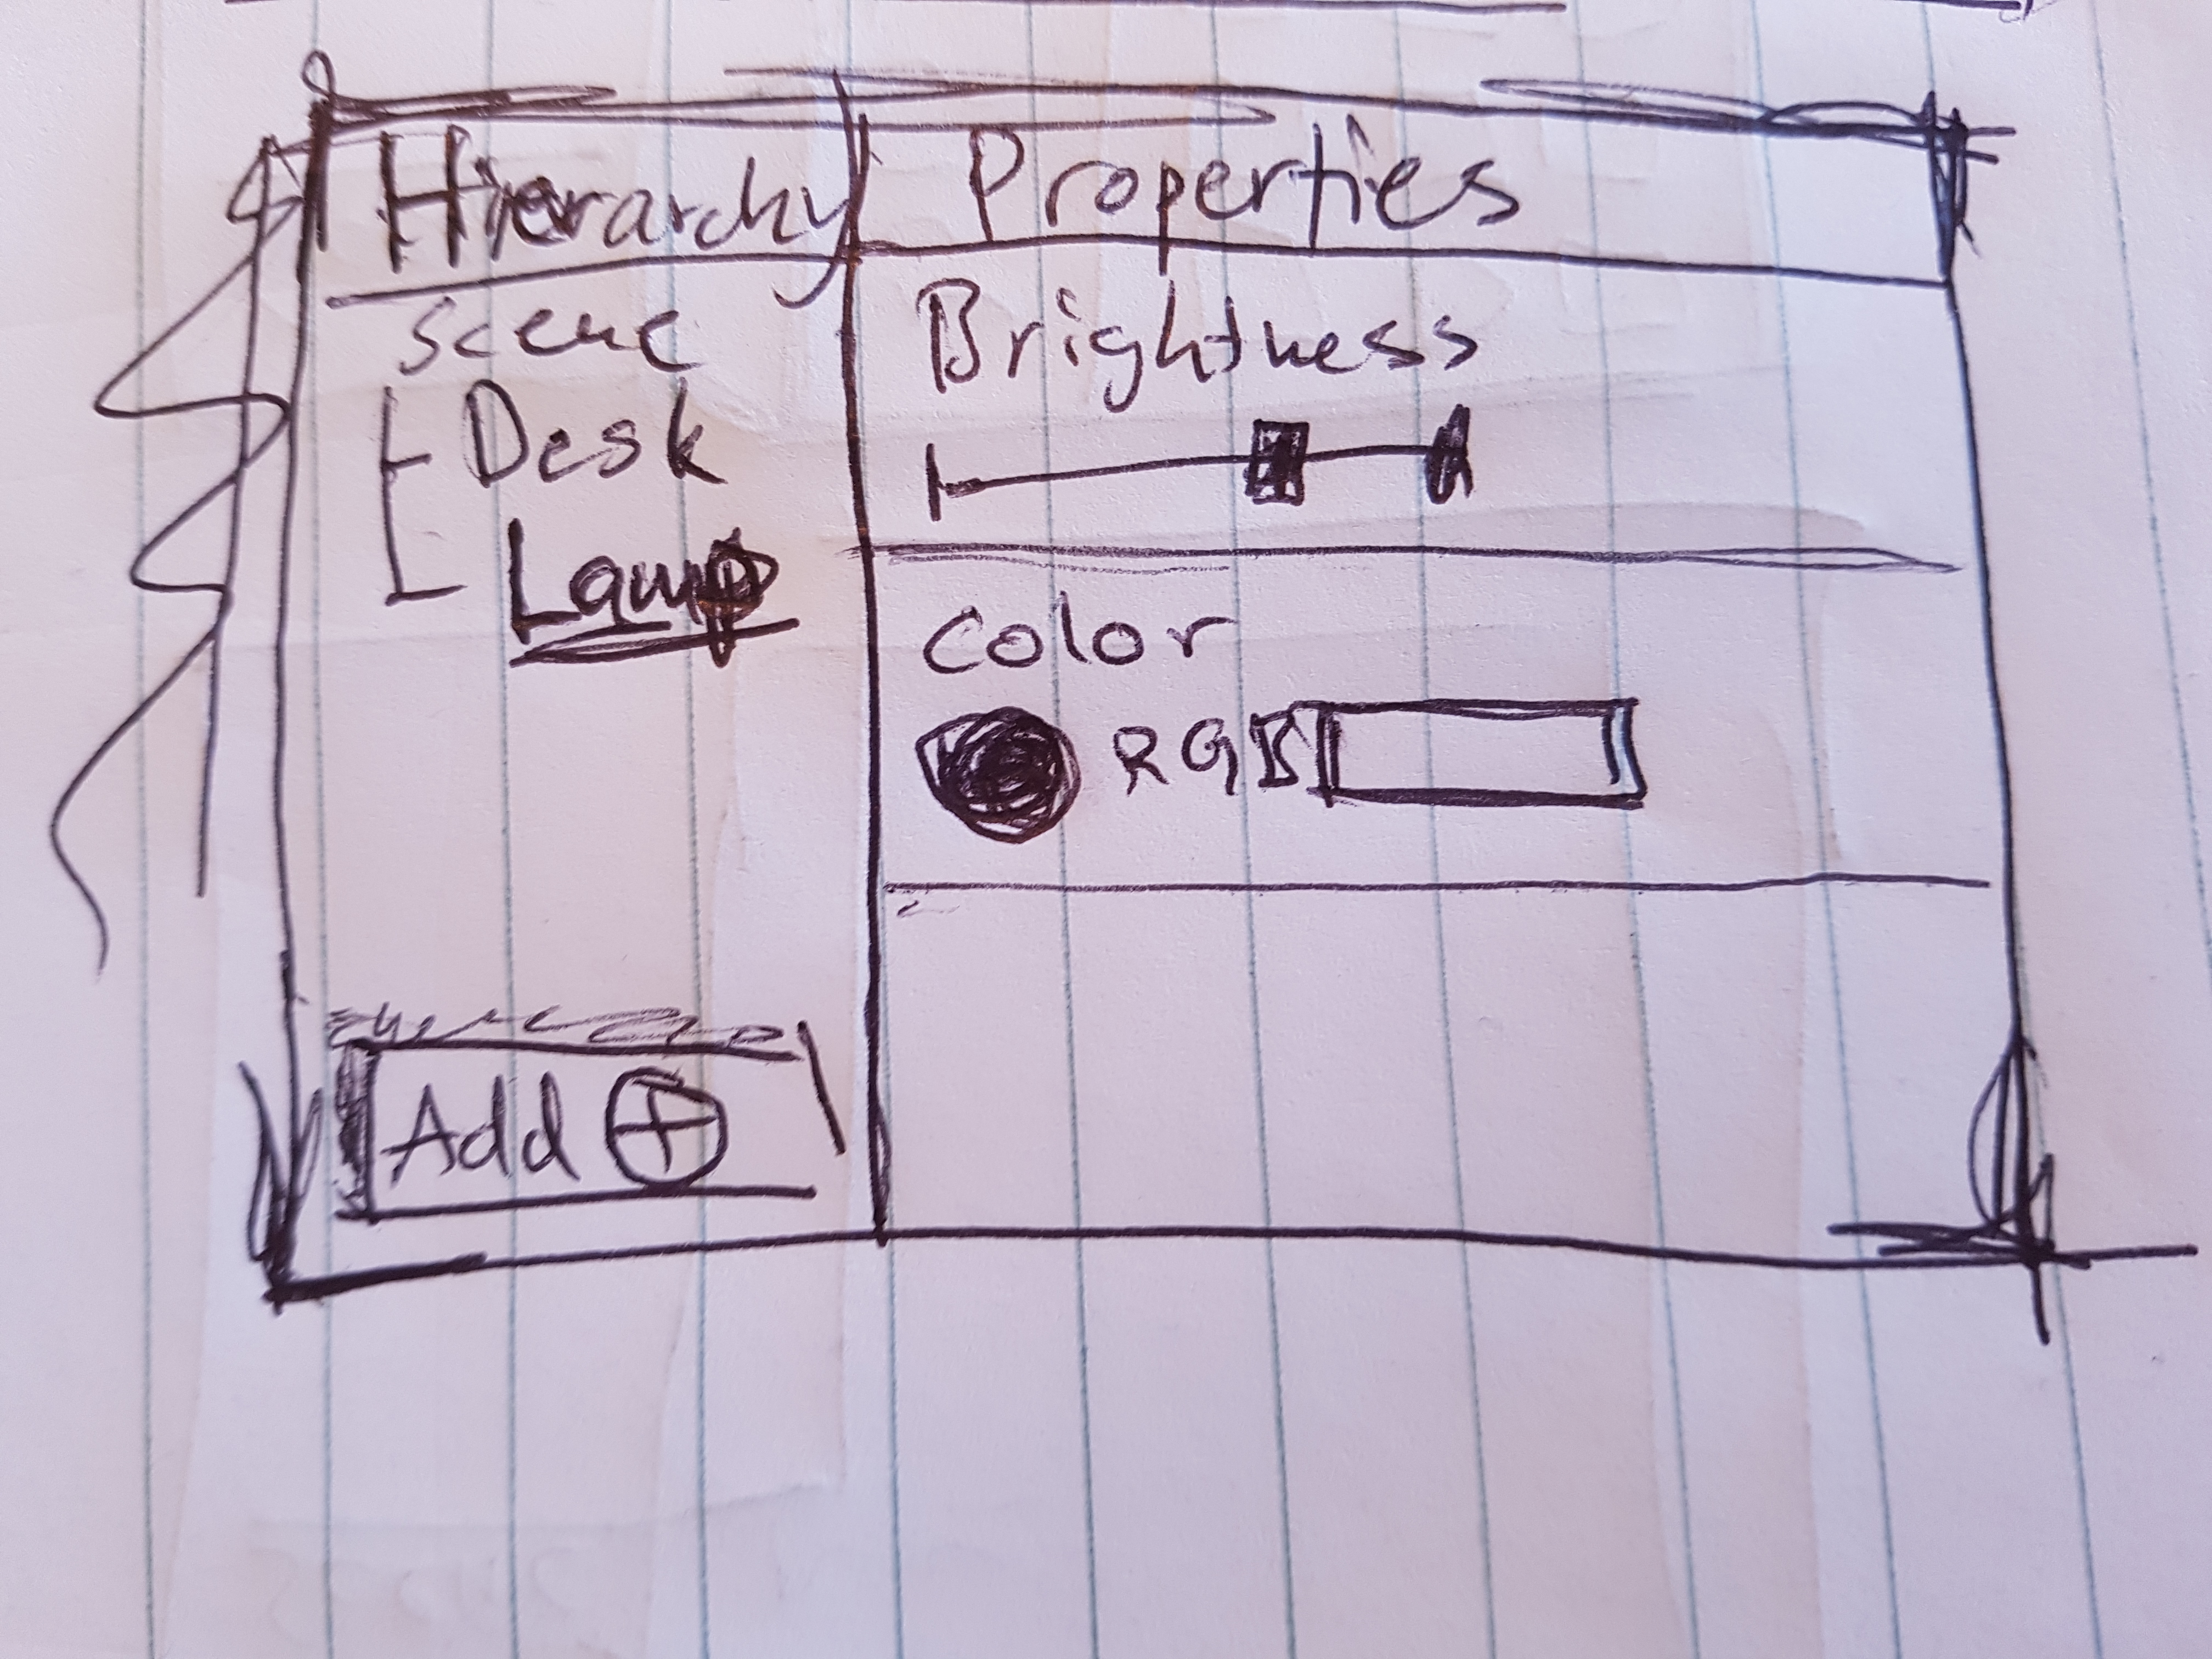
\includegraphics[width=.8\linewidth]{lo-fi/belt-props.jpg}
  \caption{A selection of objects that can be added to the VE}
  \label{fig:lofi:belt-ui:add}
\end{subfigure}
\caption{Paper sketches of the primary UI of the tool: Belt UI}
\label{fig:lofi:belt-ui}
\end{figure}

%% ********* FIELD-OF-VIEW IMAGES **********

\begin{figure}
  \begin{subfigure}{.5\textwidth}
  \centering
  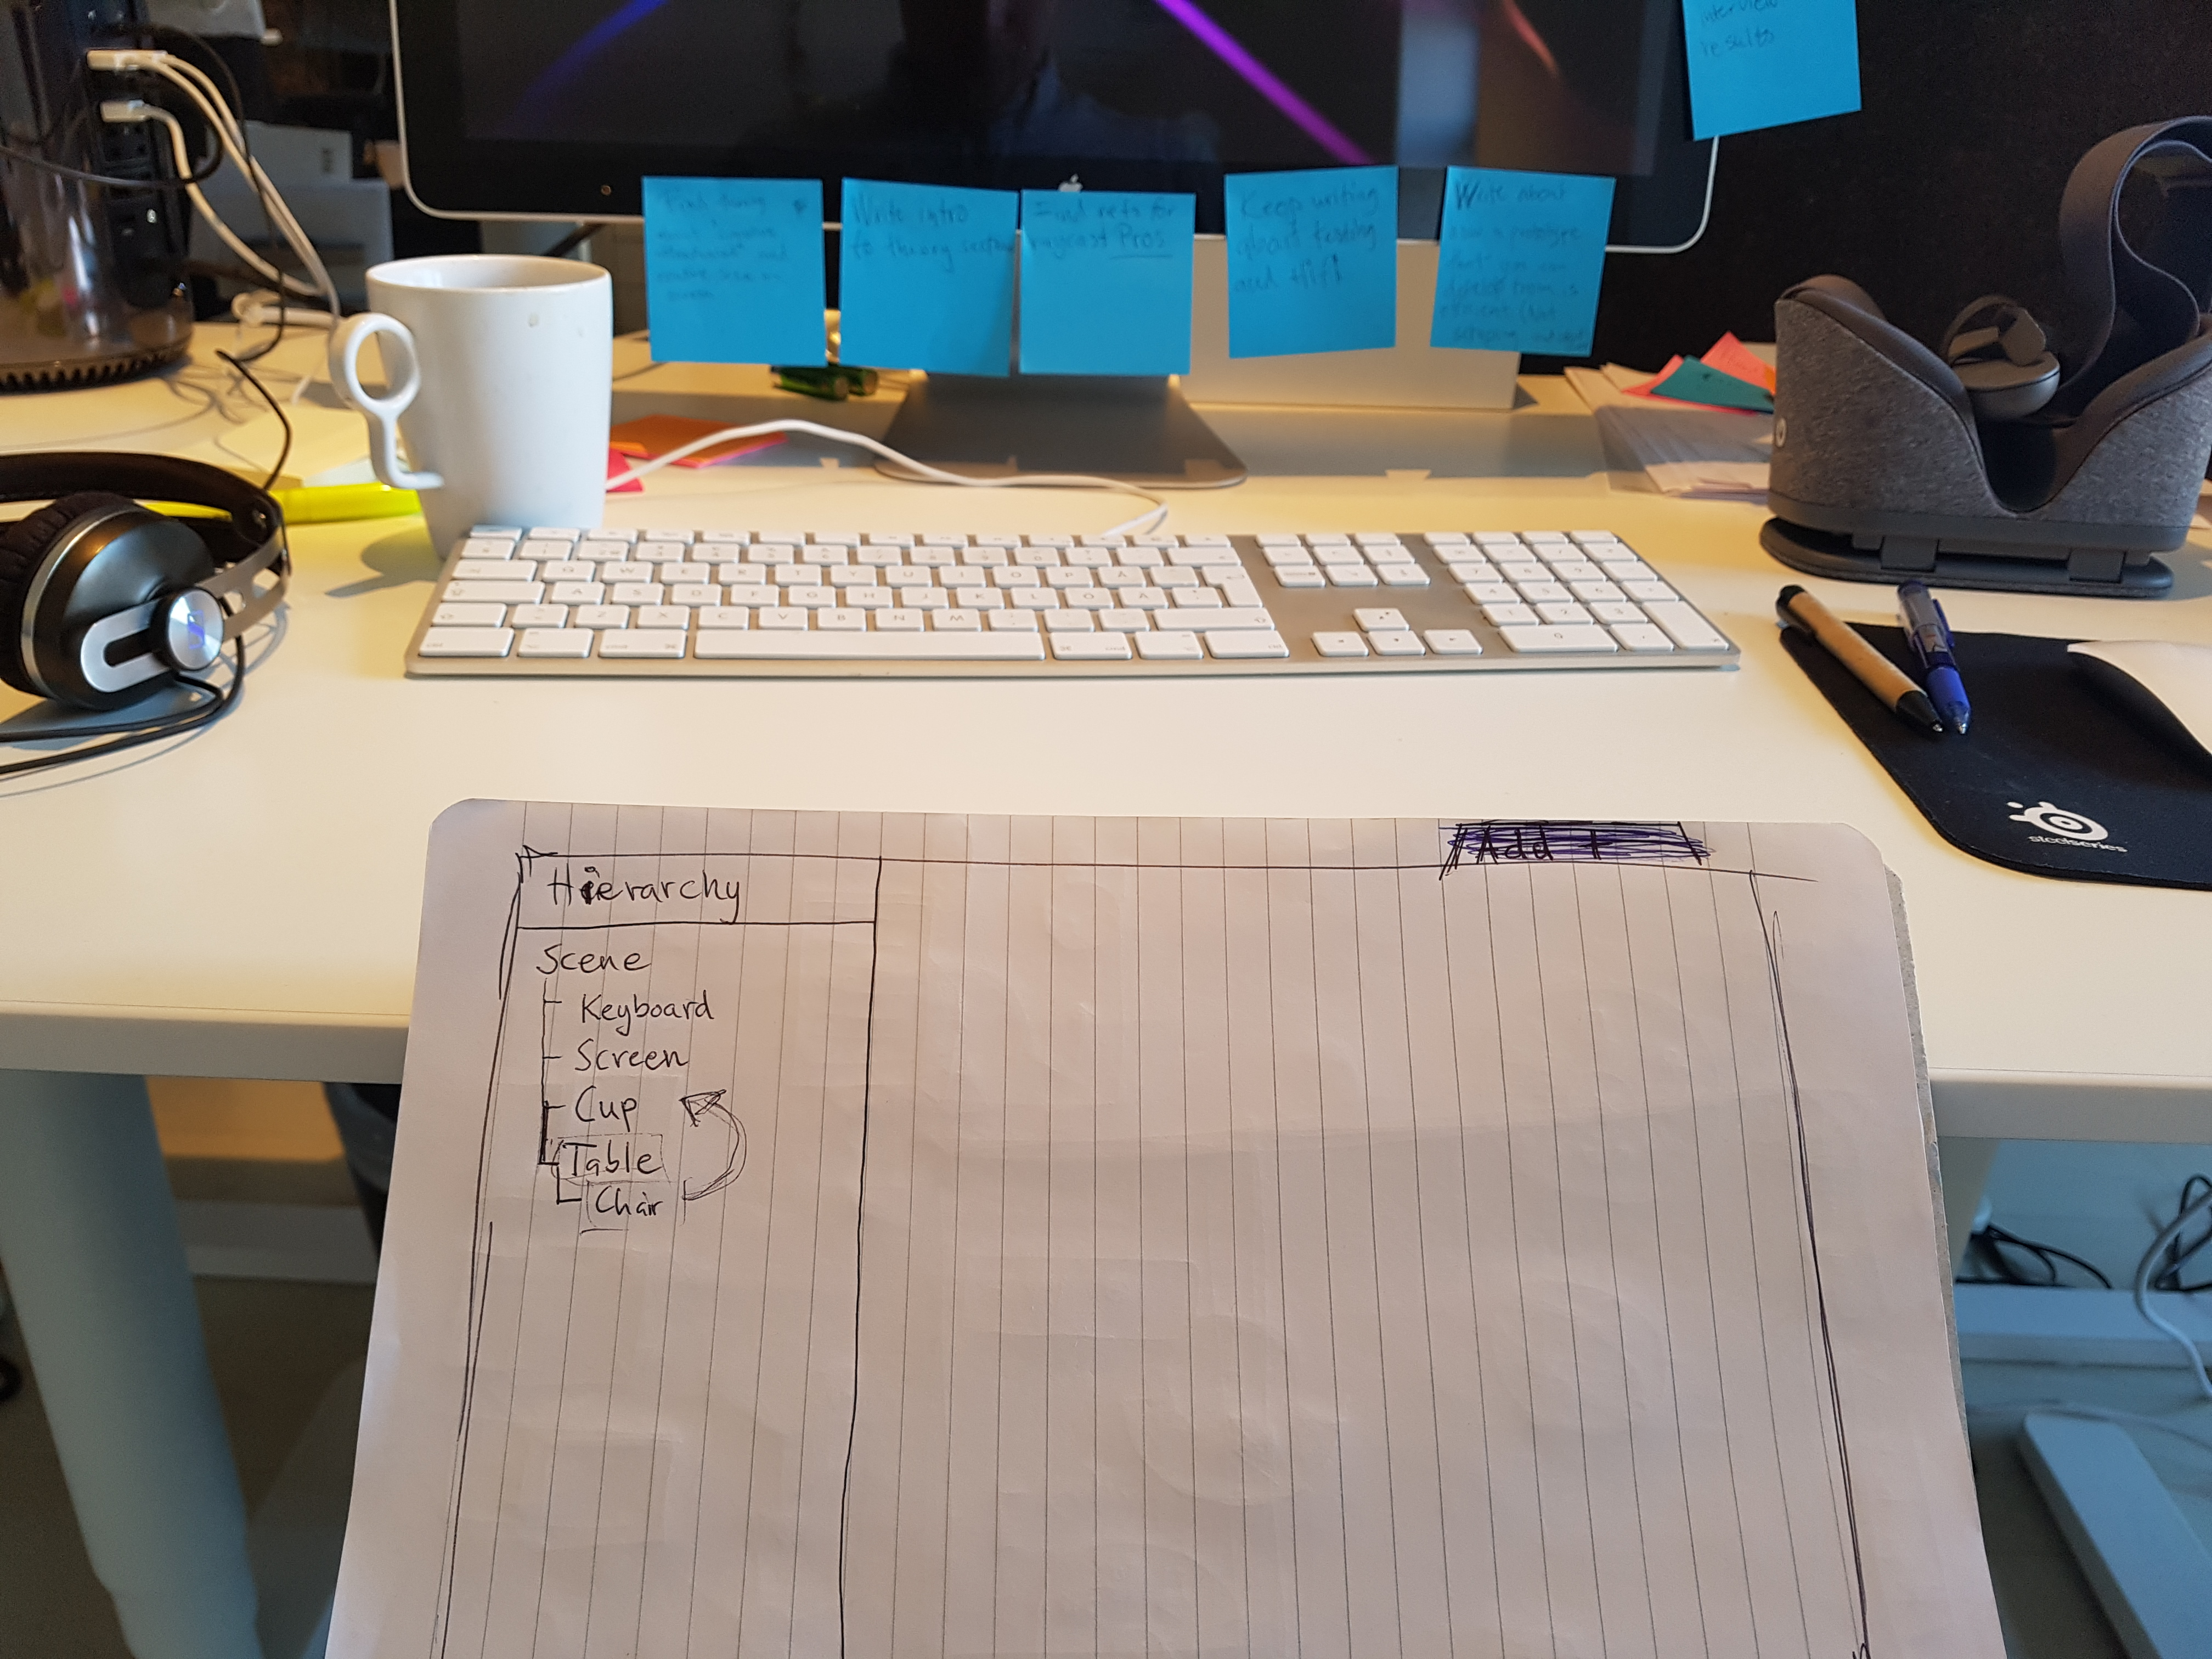
\includegraphics[width=.8\linewidth]{lo-fi/belt-perspective.jpg}
  \caption{Field of view for the user with the belt UI open}
  \label{fig:lofi:fov:belt-ui}
  \end{subfigure}%
  \begin{subfigure}{.5\textwidth}
    \centering
    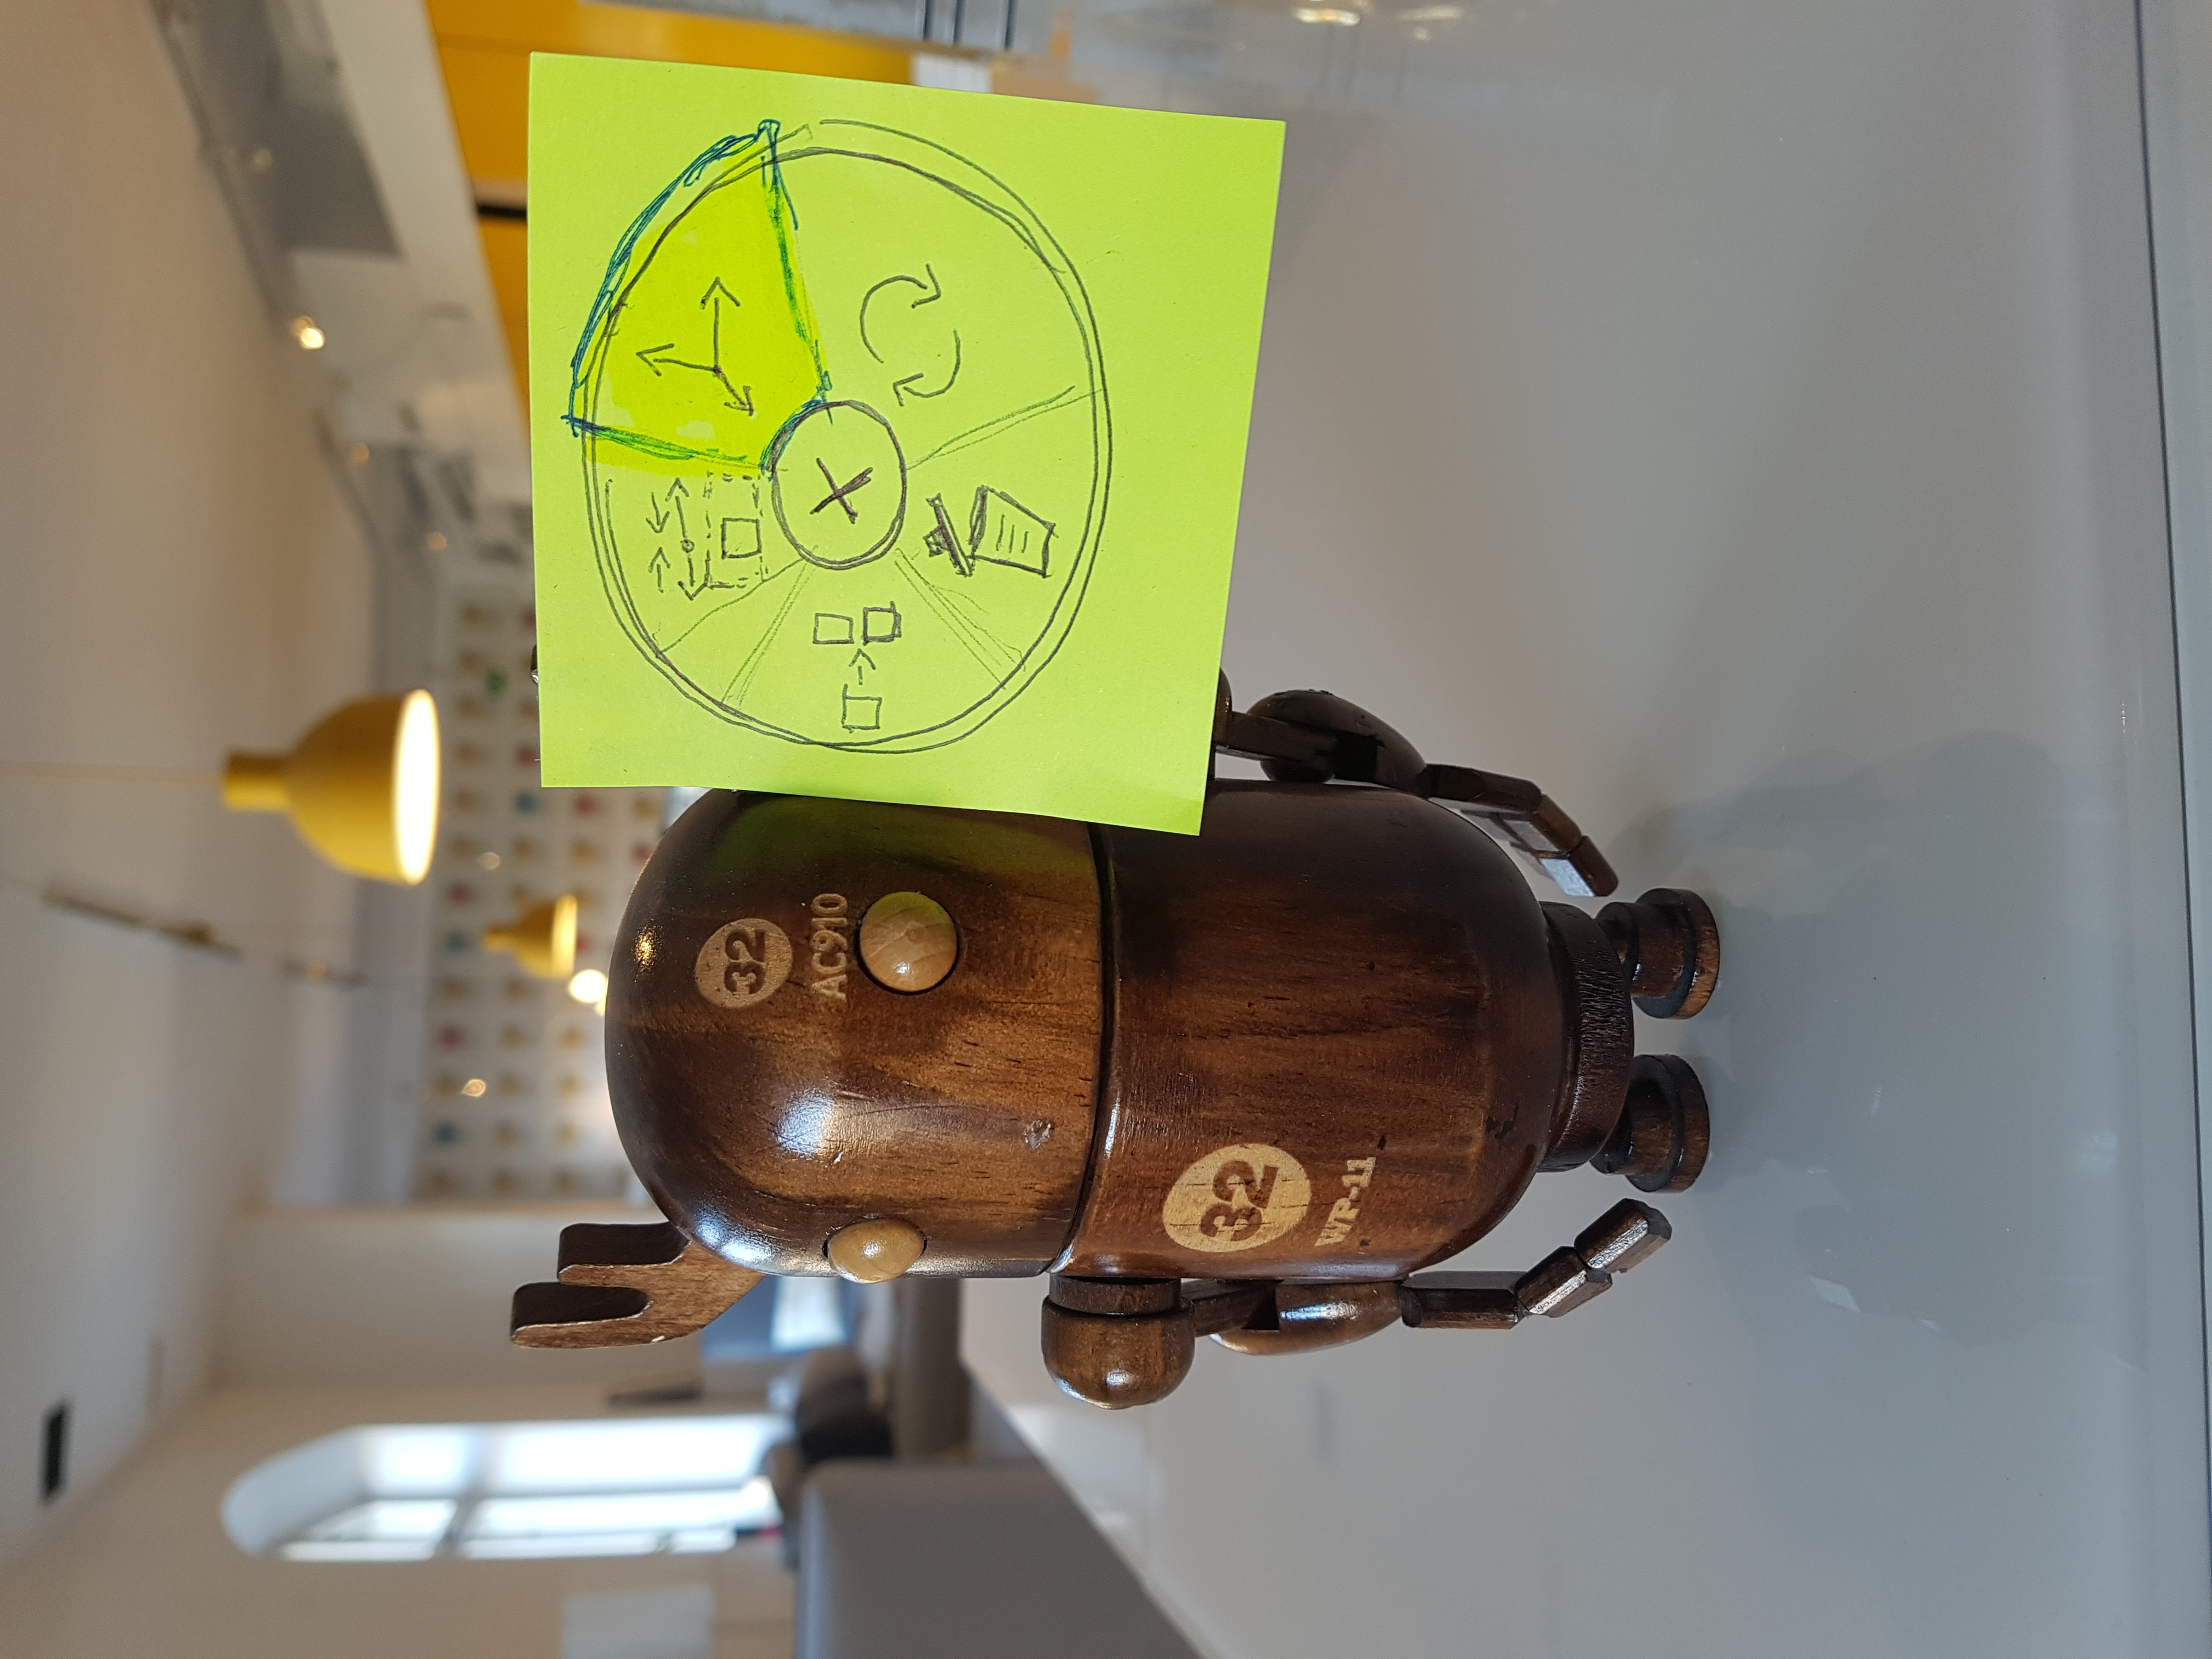
\includegraphics[width=.8\linewidth]{lo-fi/selector-perspective.jpg}
    \caption{Field of view for the user with a visible selector}
    \label{fig:lofi:fov:selector}
\end{subfigure}
\caption{Field of view for the user with different parts of the UI}
\label{fig:lofi:fov}
\end{figure}

%% ********* SELECTOR IMAGES **********

\begin{figure}
\begin{subfigure}{.5\textwidth}
  \centering
  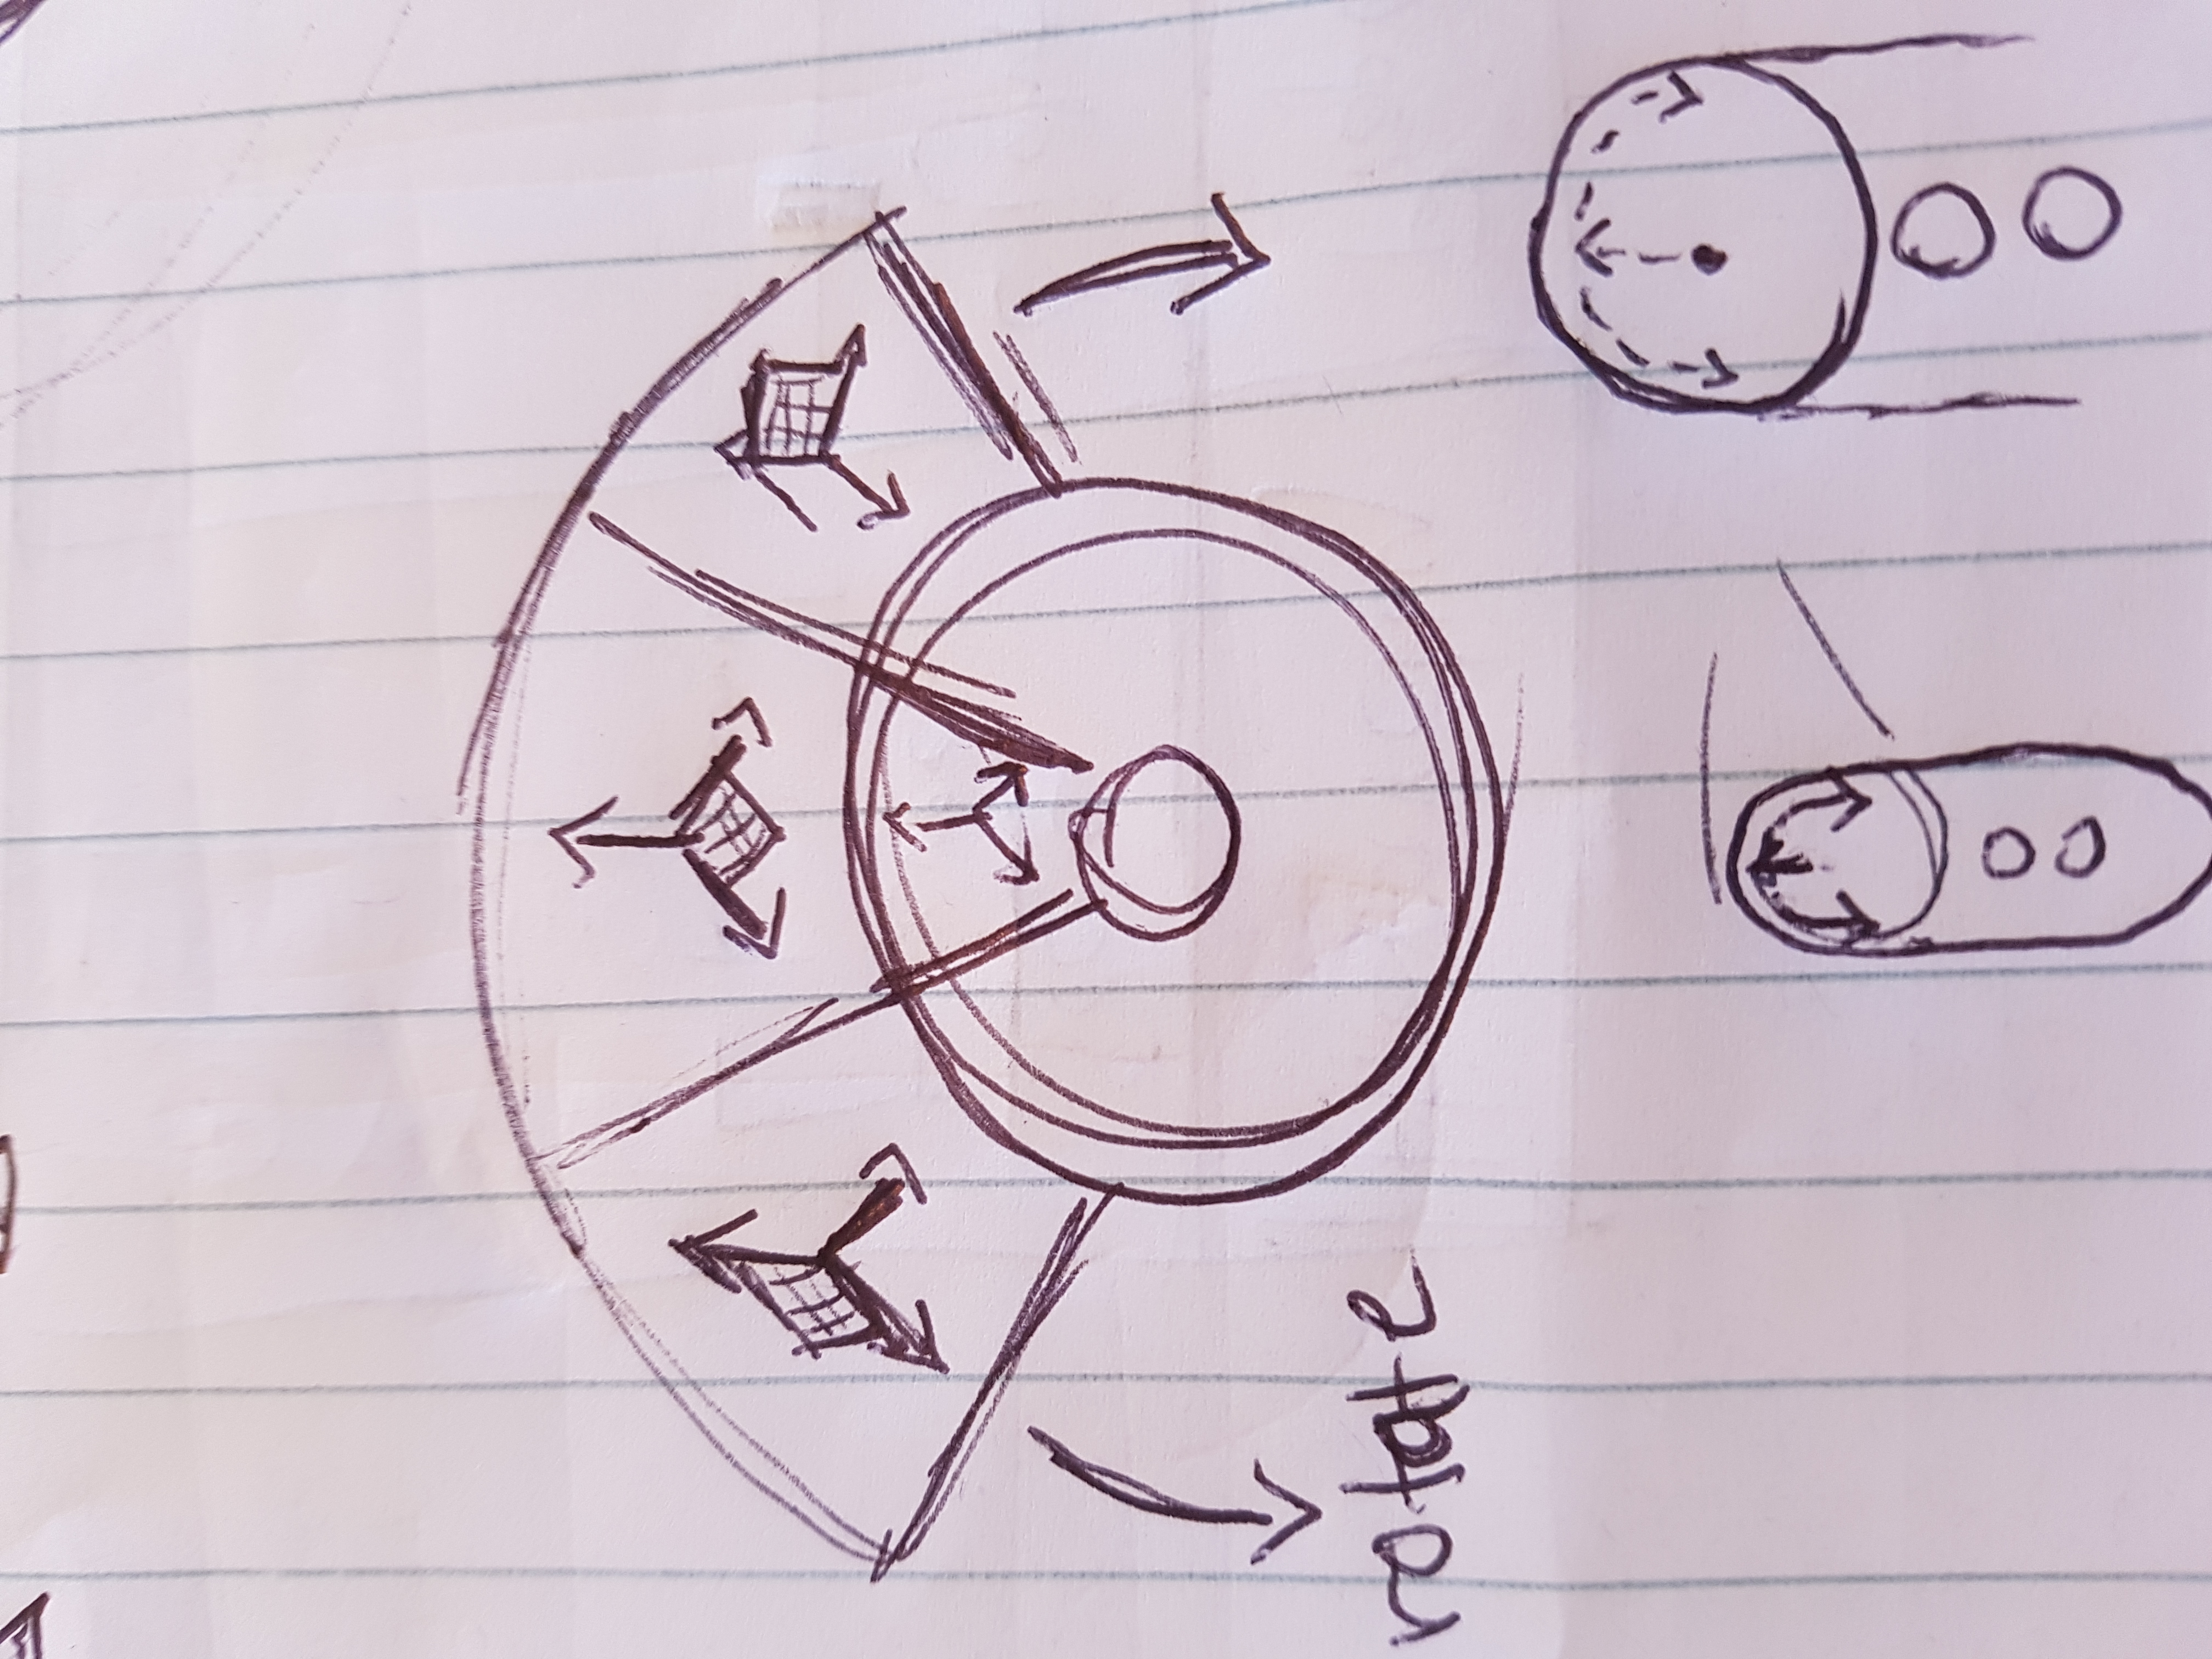
\includegraphics[width=.8\linewidth]{lo-fi/selector-submenu.jpg}
  \caption{Accessing a submenu of the selector}
  \label{fig:lofi:selector:select}
\end{subfigure}%
\begin{subfigure}{.5\textwidth}
  \centering
  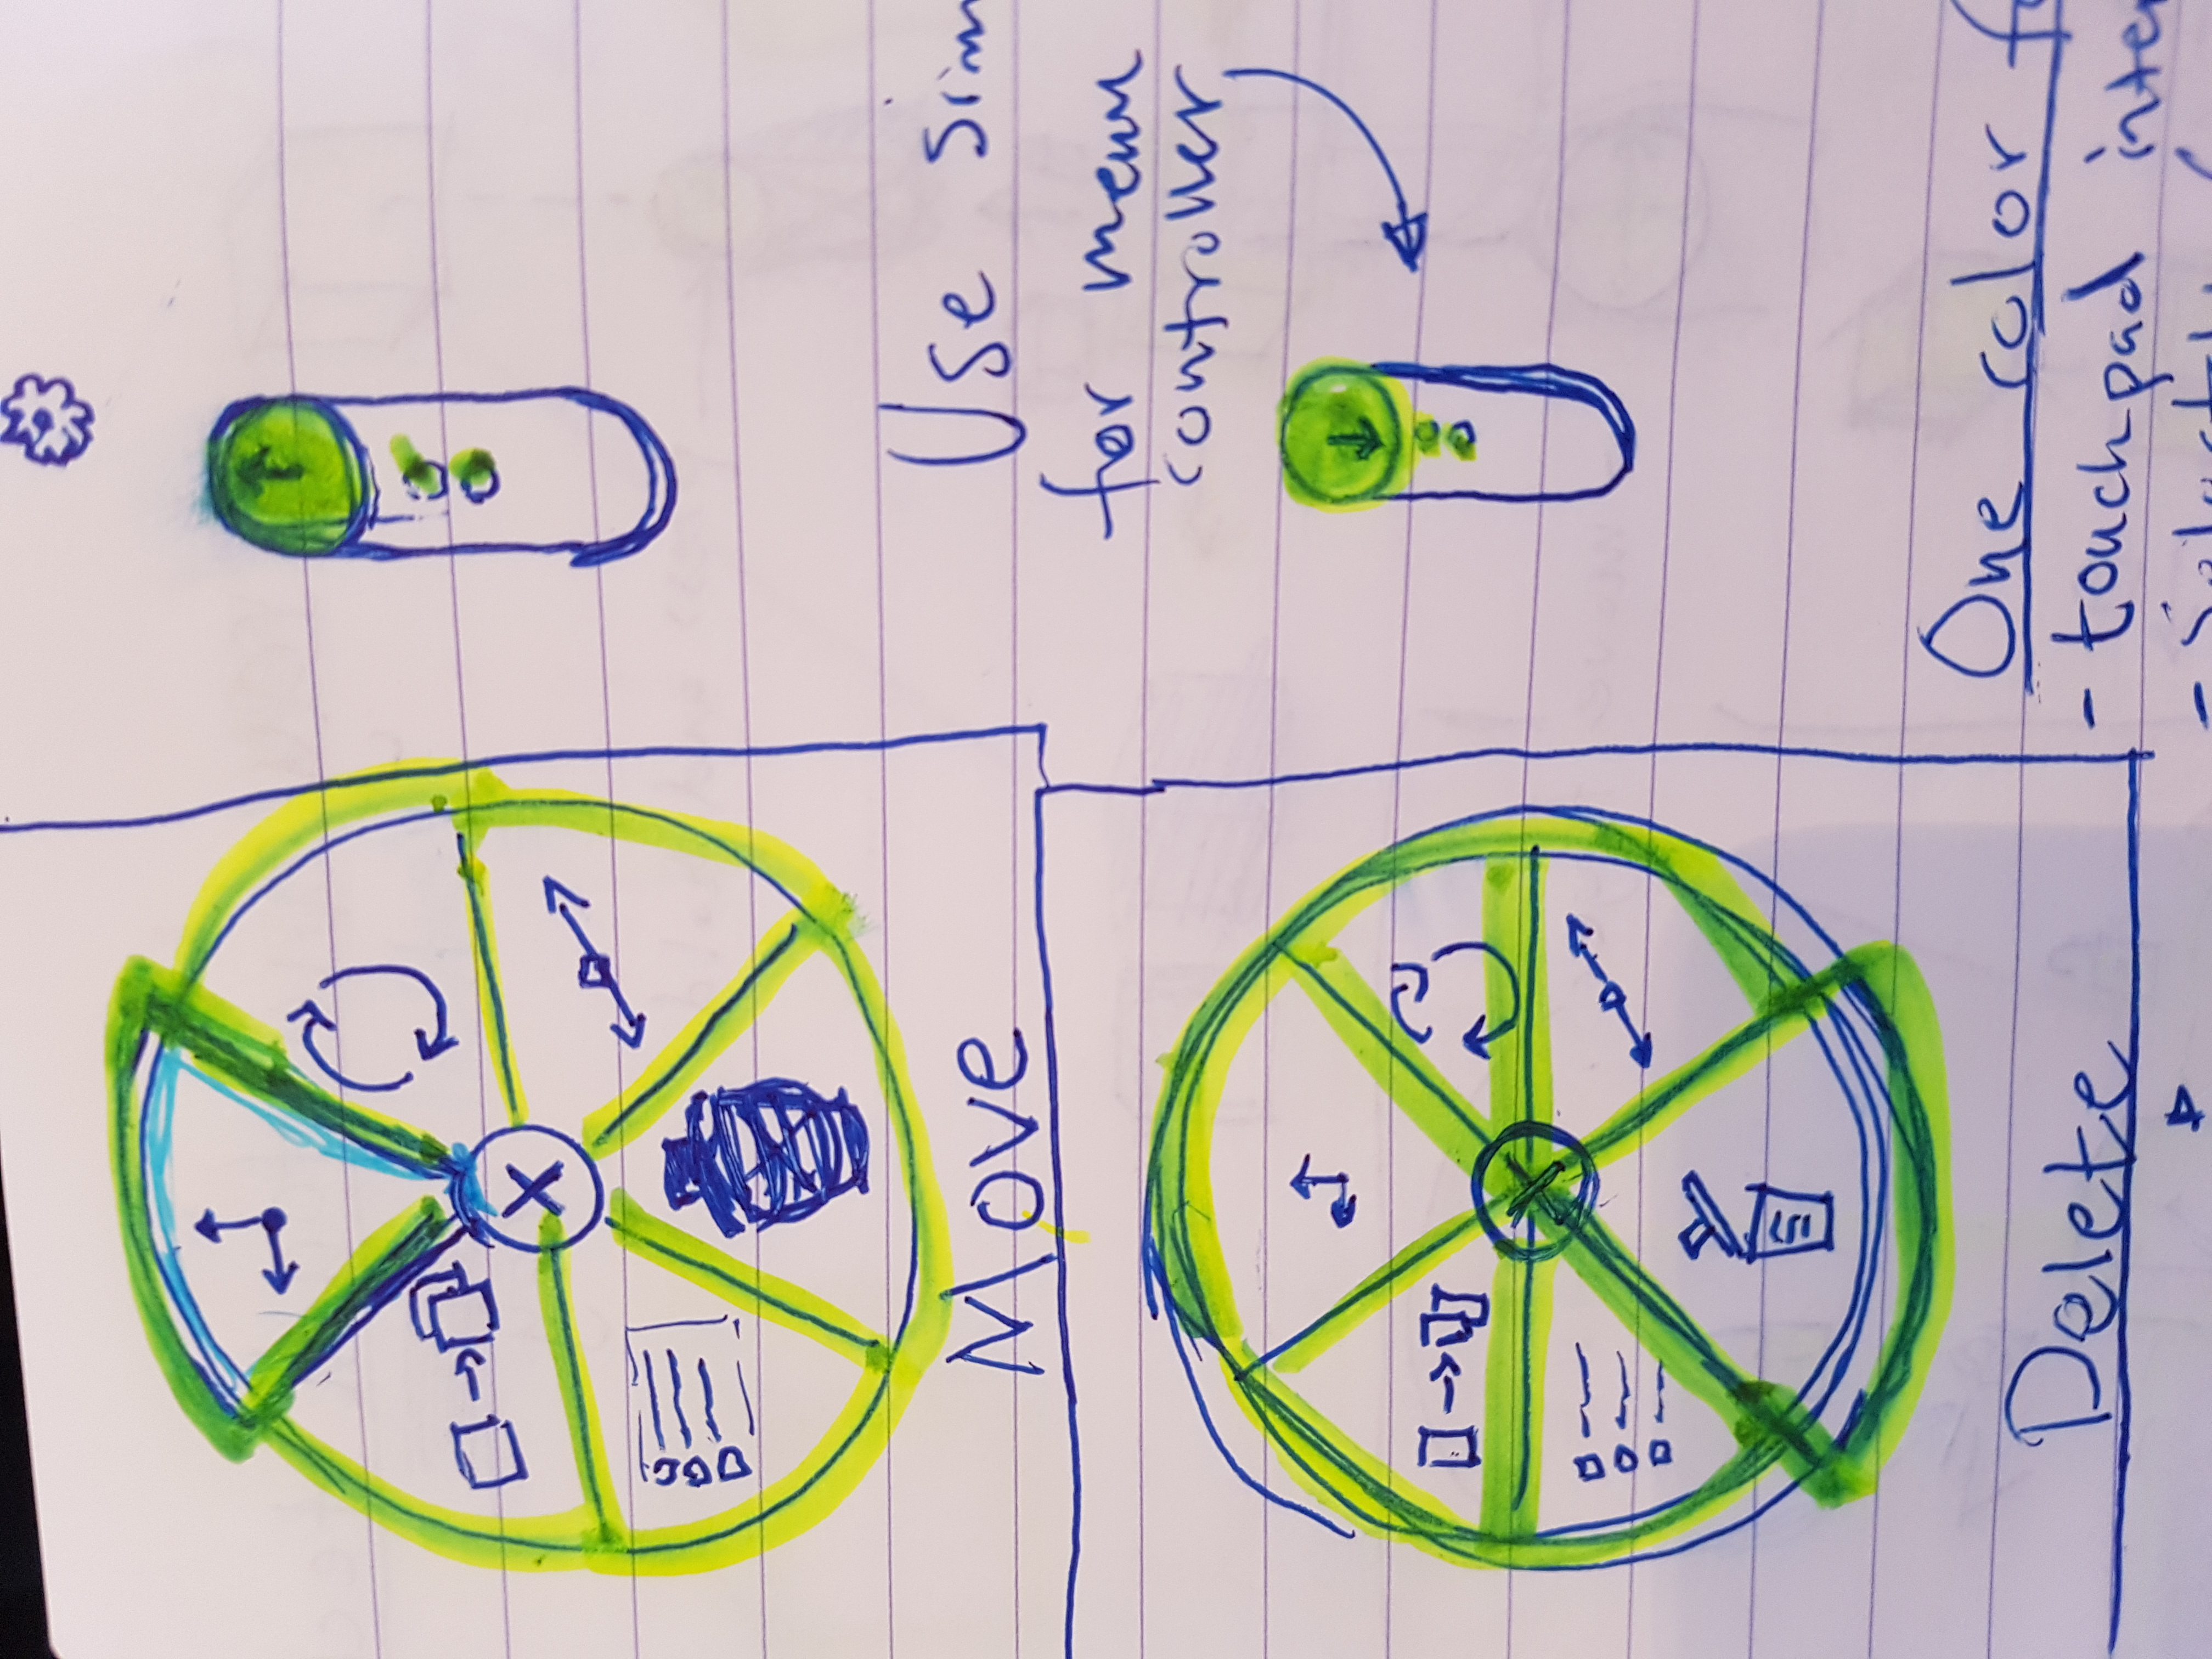
\includegraphics[width=.8\linewidth]{lo-fi/selector-select.jpg}
  \caption{selection in the selector}
  \label{fig:lofi:selector:submenu}
\end{subfigure}
\caption{Multilevel menu selector for objects}
\label{fig:lofi:selector}
\end{figure}

%% ********* BELT UI IMAGES **********

\begin{figure}
\begin{subfigure}{.5\textwidth}
  \centering
  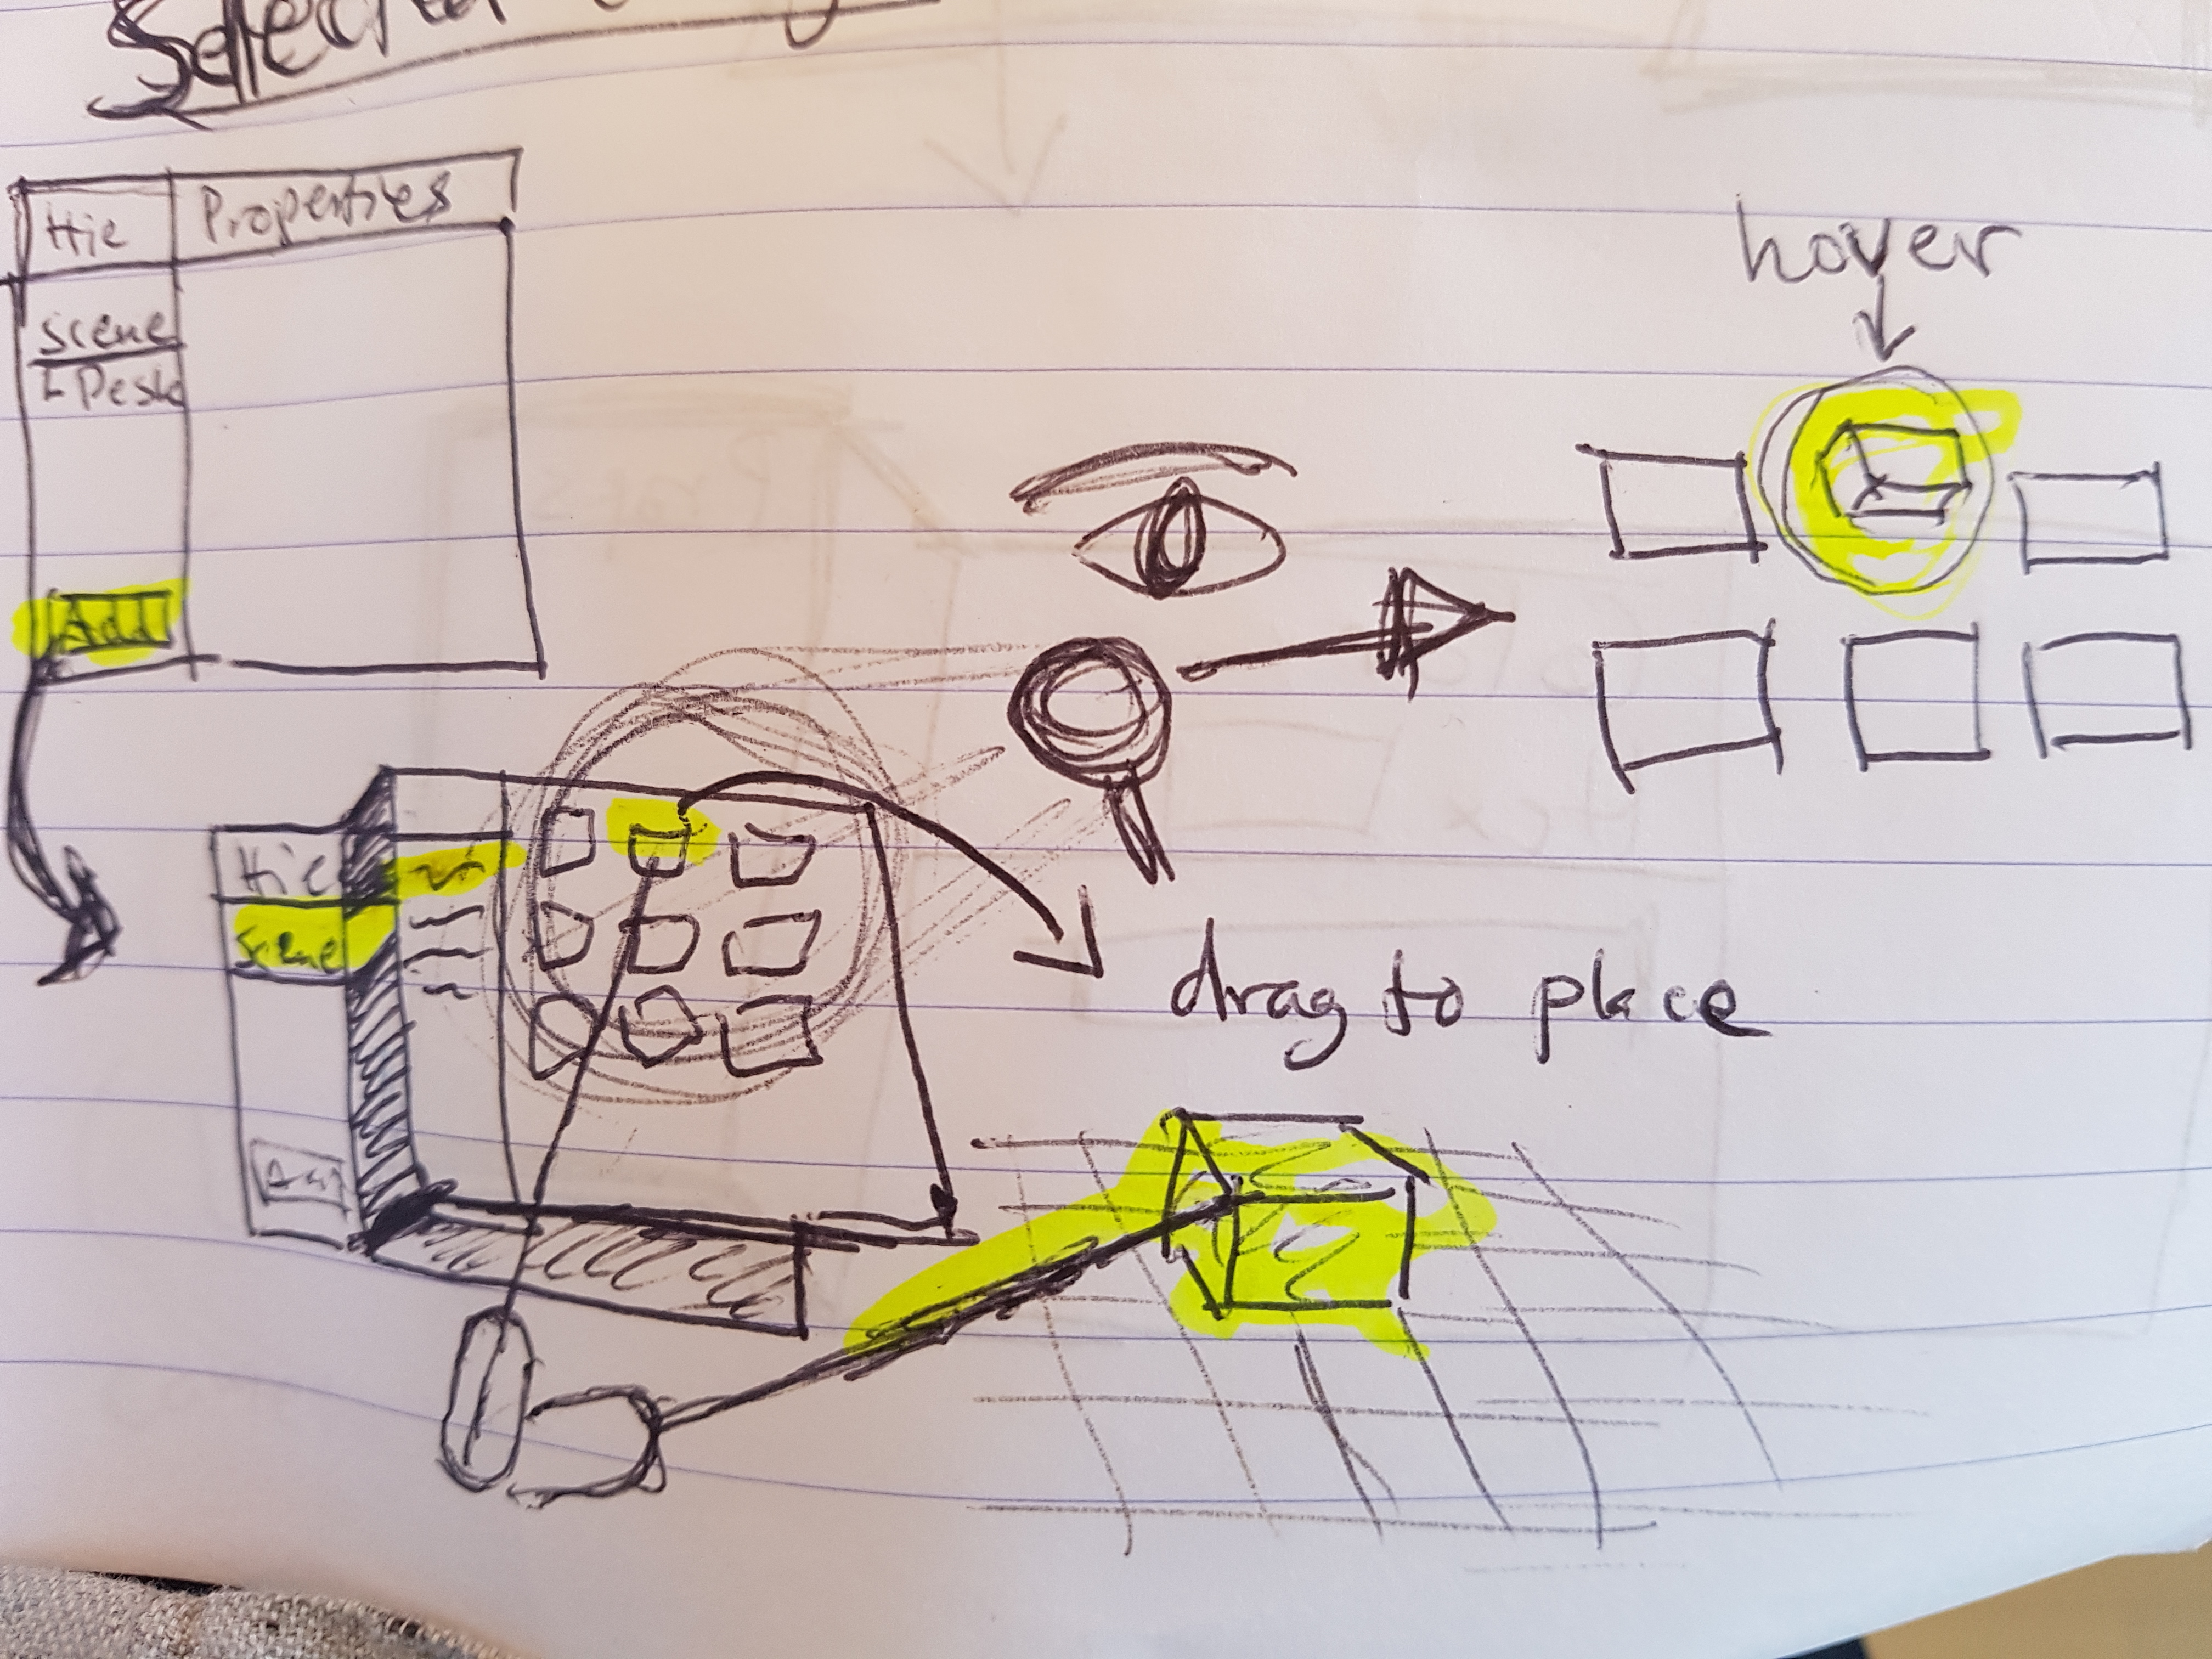
\includegraphics[width=.8\linewidth]{lo-fi/add-object.jpg}
  \caption{Properties of a selected object in the belt UI}
  \label{fig:lofi:object:add}
\end{subfigure}%
\begin{subfigure}{.5\textwidth}
  \centering
  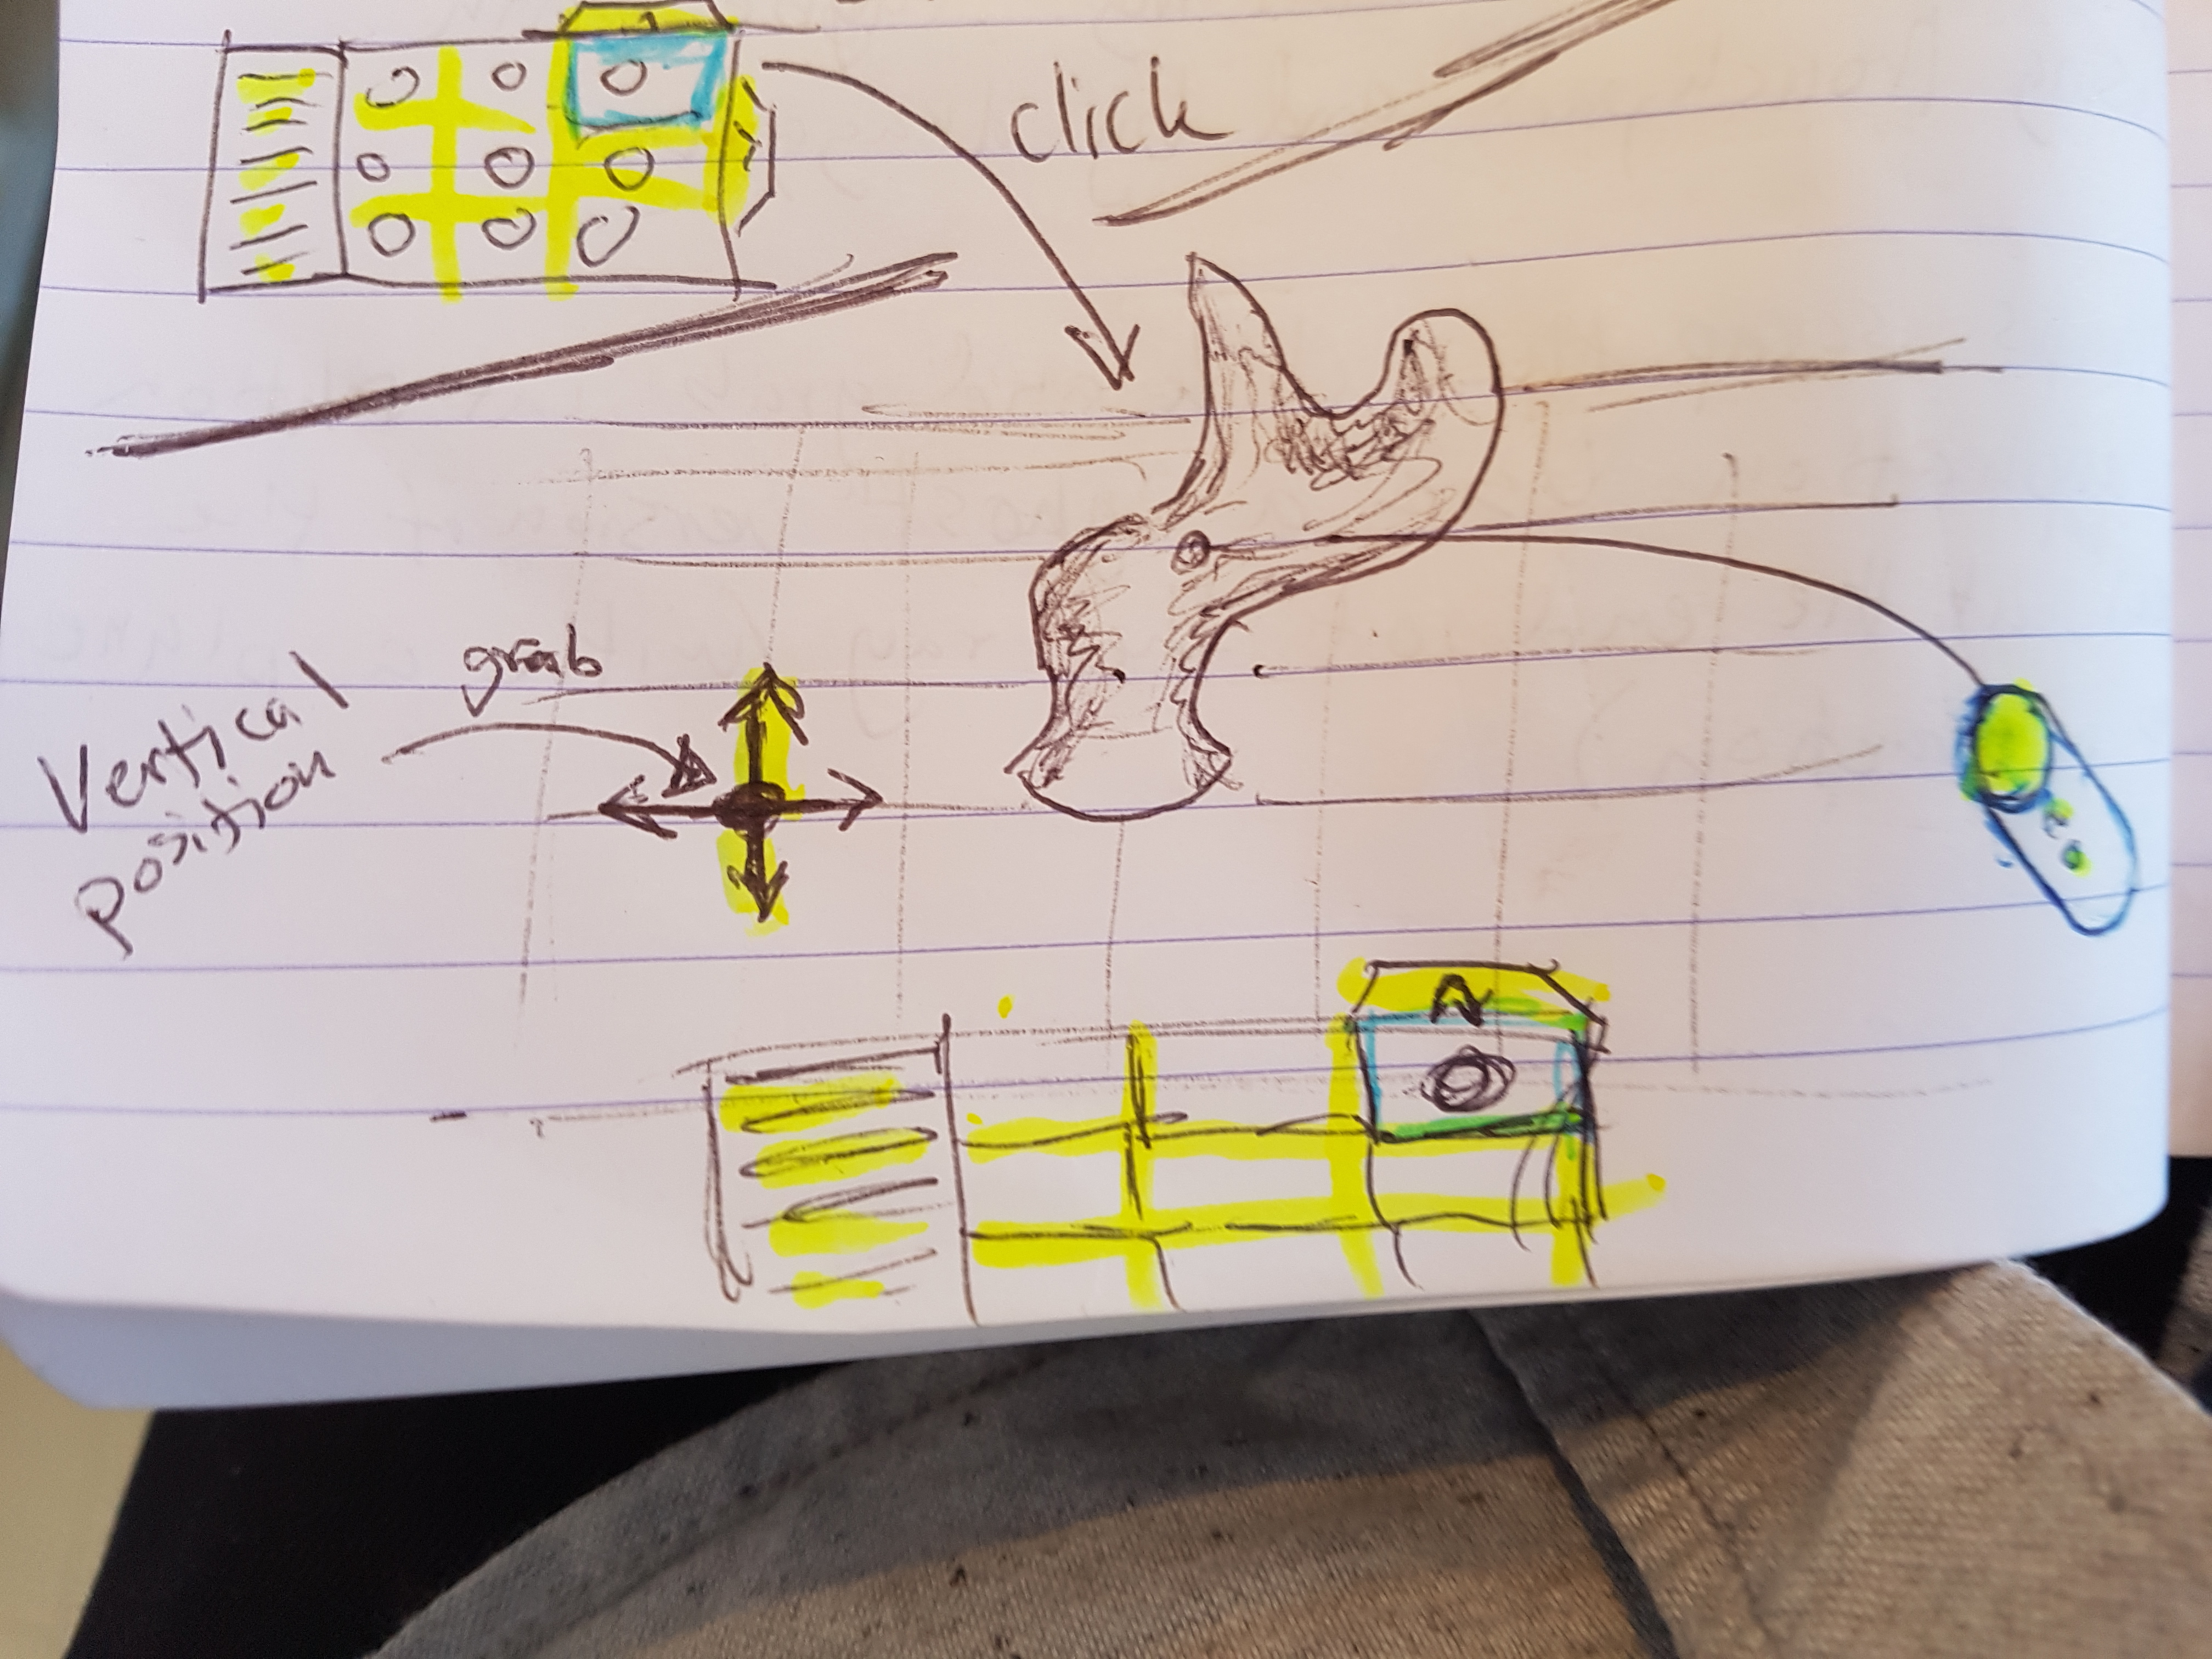
\includegraphics[width=.8\linewidth]{lo-fi/move-object.jpg}
  \caption{A selection of objects that can be added to the VE}
  \label{fig:lofi:object:move}
\end{subfigure}
\caption{Paper sketches of the primary UI of the tool: Belt UI}
\label{fig:lofi:object}
\end{figure}

%% ********* TILT BRUSH SKETCHES **********

\begin{figure}
\begin{subfigure}{.5\textwidth}
  \centering
  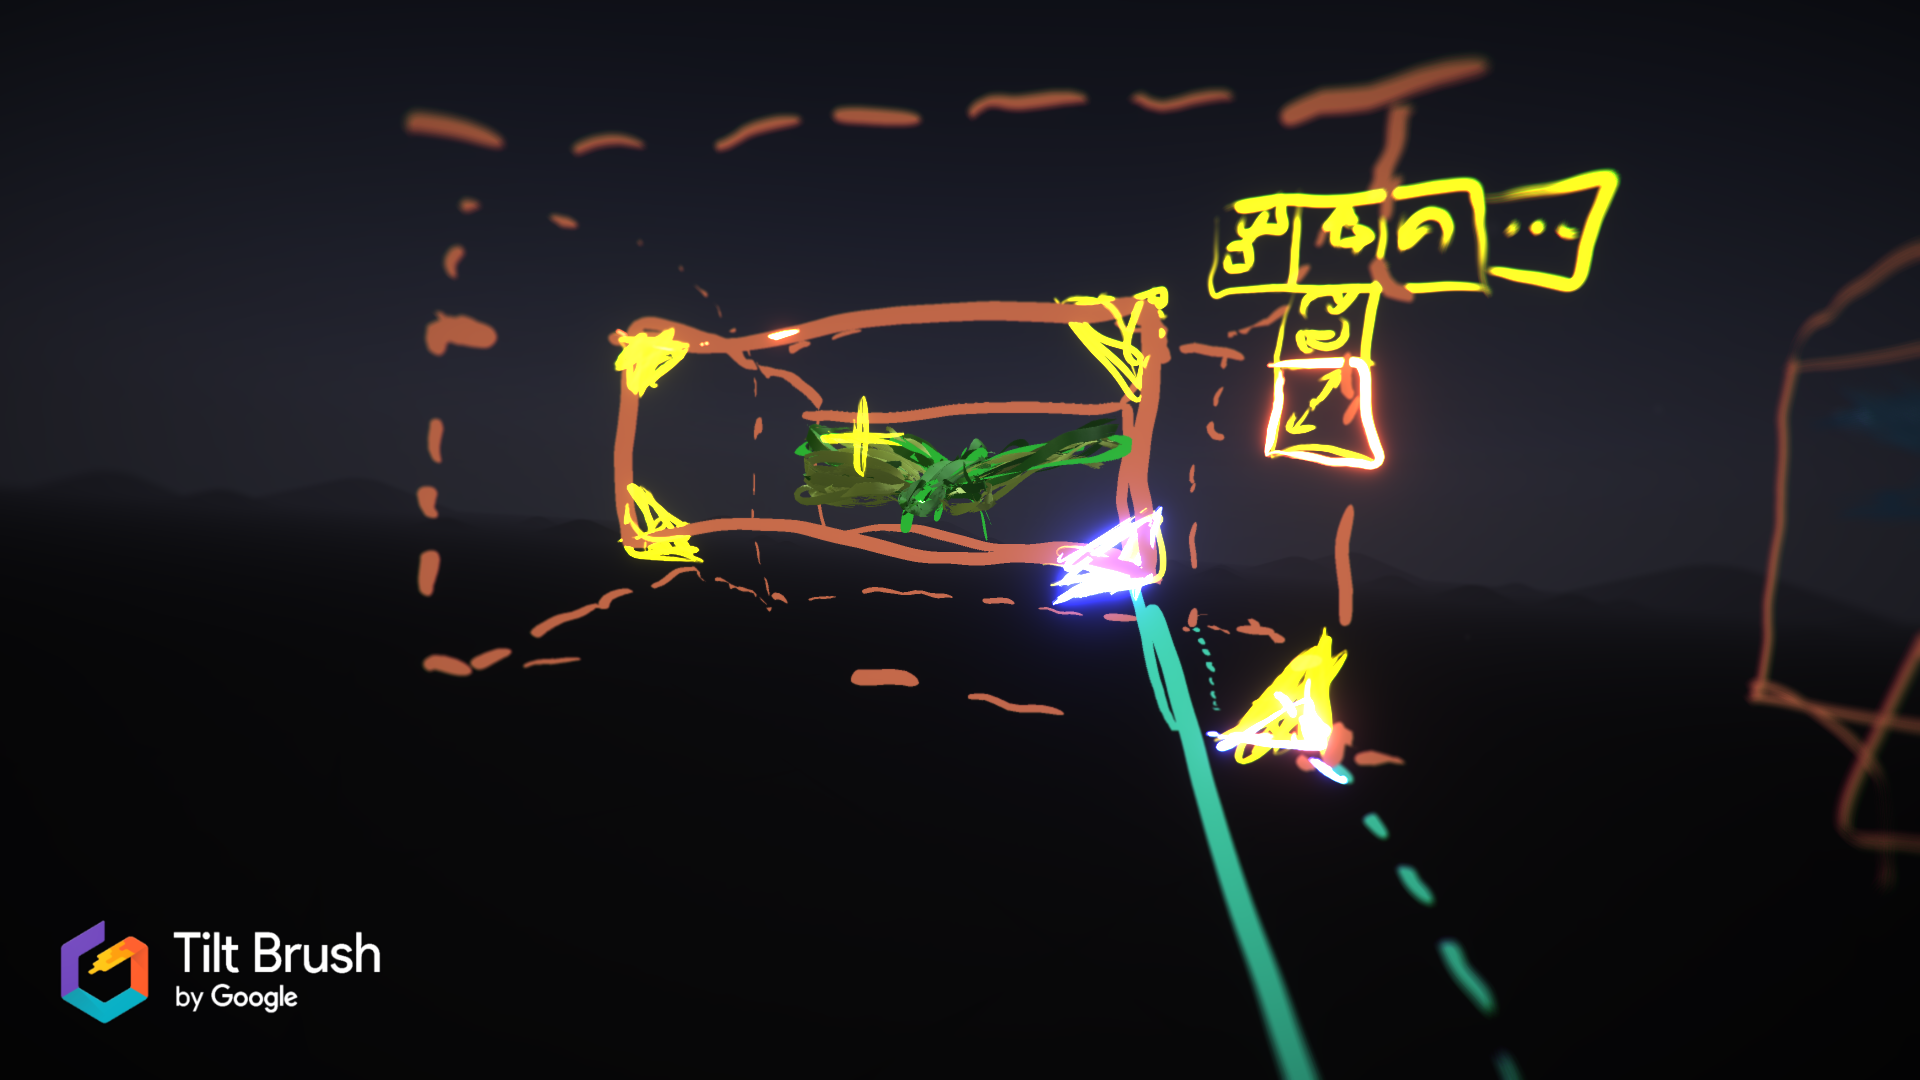
\includegraphics[width=.8\linewidth]{lo-fi/scalescenario3.PNG}
  \caption{A scale scenario where bottom right corner of a boundingbox is moved}
  \label{fig:lofi:tilt:scale3}
\end{subfigure}%
\begin{subfigure}{.5\textwidth}
  \centering
  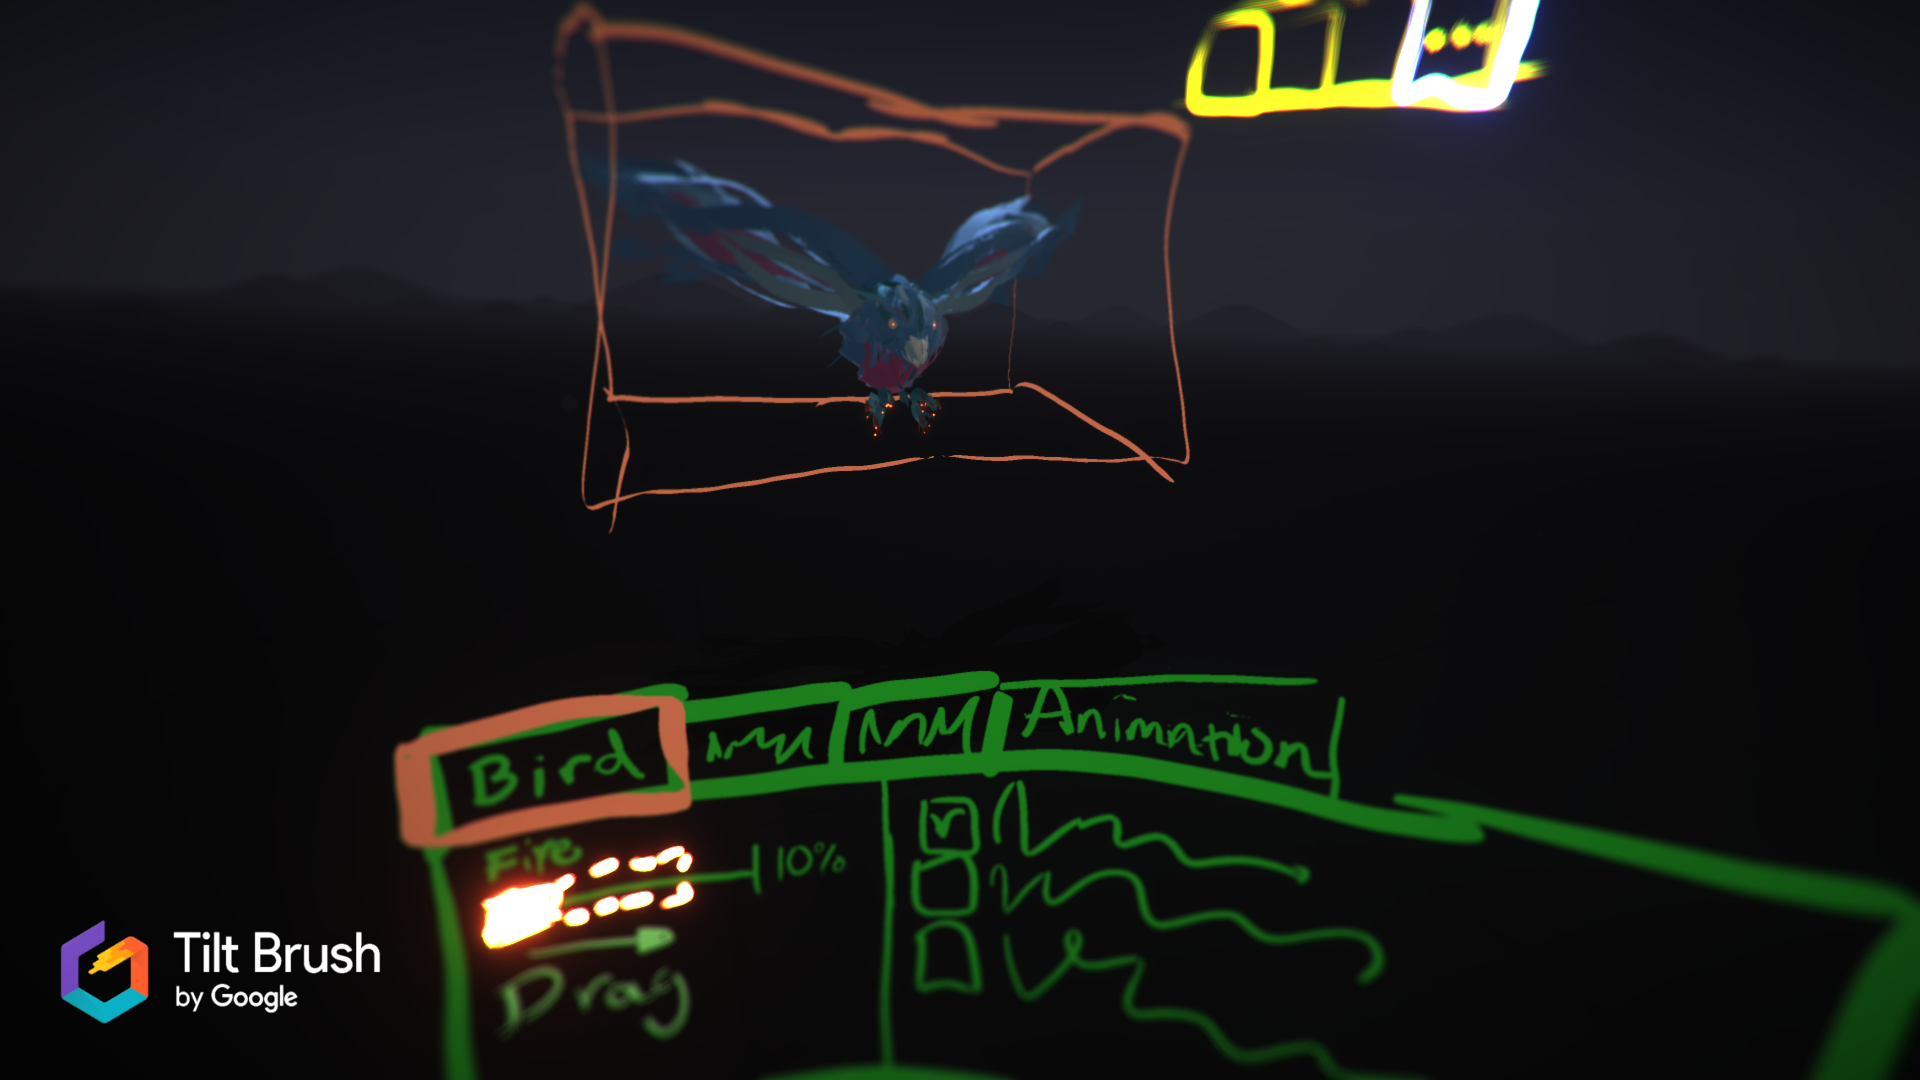
\includegraphics[width=.8\linewidth]{lo-fi/birdmenu2.PNG}
  \caption{Accessing properties of an object}
  \label{fig:lofi:tilt:passivemenu}
\end{subfigure}
\caption{Lo-fi sketches. Created in Tilt Brush (see Section \ref{relatedwork:tiltbrush})}
\label{fig:lofi:tilt}
\end{figure}
